../../hw03/report/pcsmacros.tex
\include{pythonlisting}

\huge
\pgfdeclareimage[height=0.85in]{mypic}{esteban}
\linethickness{0.2mm}

\title[]{CIP wavefield tomography with illumination compensation }
\author[]{Esteban  D\'{i}az$^{*}$ and Paul Sava}
\institute{Center for Wave Phenomena, 
Colorado School of Mines 
 \\ \pgfuseimage{mypic}}
\date{}
\logo{}


\def\big#1{\begin{center} \LARGE \textbf{#1} \end{center}}
\def\cen#1{\begin{center}        \textbf{#1} \end{center}}

\tikzstyle{arrow}=[draw, -latex] 
\tikzstyle{rarrow}=[arrow,line width=.8mm,draw=red, fill=red]
\tikzstyle{karrow}=[arrow,scale=.5,line width=.8mm,draw=black, fill=black]
\tikzstyle{RectObject}=[rectangle,fill=white,draw,line width=0.5mm]

% ------------------------------------------------------------
\mode<beamer> { \cwpcover }

\inputdir{ximages}

\begin{frame}
  
\end{frame}



\inputdir{gauss_images}
\begin{frame}
  \[
     R(\xx) =
     \sum_{t} u_s(\xx,t) u_r(\xx,t)
  \]
\sep  
  \itab{$u_s$: source wavefield} \\ 
  \itab{$u_r$: receiver wavefield}\\
  \white{\itab{$\hh,\tau$: space and time-lags}}  
\end{frame}


\begin{frame}
  \[
     R(\xx,\hh,\tau) =
     \sum_{t} u_s(\xx+\hh,t+\tau) u_r(\xx-\hh,t-\tau)
  \]
\sep  
  \itab{$u_s$: source wavefield} \\ 
  \itab{$u_r$: receiver wavefield}\\
  \itab{$\hh,\tau$: space and time-lags}  
\end{frame}

\begin{frame}
  \[
     R(\red{\xx},\hh,\tau) =
     \sum_{t} u_s(\red{\xx}+\hh,t+\tau) u_r(\red{\xx}-\hh,t-\tau)
  \]
\sep  
  \itab{$u_s$: source wavefield} \\ 
  \itab{$u_r$: receiver wavefield}\\
  \itab{$\hh,\tau$: space and time-lags}  

\end{frame}

\begin{frame}
  \[
     R(\xx_c,\hh,\tau) =
     \sum_{t} u_s(\xx_c+\hh,t+\tau) u_r(\xx_c-\hh,t-\tau)
  \]
\sep  
  \itab{$u_s$: source wavefield}\\
  \itab{$u_r$: receiver wavefield}\\
  \itab{$\hh,\tau$: space and time-lags}  
\end{frame}


\begin{frame}
  \begin{align}
    {\bf R}_{\hh,\tau} &= {\bf I_r} {\bf u_s}  \nonumber \\
                       &=  {\bf I_s} {\bf u_r} \nonumber
  \end{align}
\sep  
  \itab{$\bf u_s$: source wavefield}\\
  \itab{$\bf u_r$: receiver wavefield}\\
  {\itab{$\hh,\tau$: space and time-lags}} 
\end{frame}
\inputdir{ximages}
\begin{frame}
  \plot{img-v100}{}{}
\end{frame}



\begin{frame}
  \[
  J(\m) = \ltnorm{P(\hh,\tau) R(\xx_c,\hh,\tau)}
  \]
\sep
  \itab{$P(\hh,\tau):$ penalty operator}\\
  \itab{$\m$: model parameter}
  \begin{flushright}
  (Yang, 2013)
  \end{flushright}
\end{frame}



\inputdir{ximages}

\begin{frame} \frametitle{penalty operator $ P(\hh,\tau)$}
  \begin{columns}
    \column{0.5\textwidth}
      \plot{pDSO-cip}{}{\klabel{95}{30}{$\sqrt{ |\hh|^2 +(v\tau)^2}$}}
    \column{0.5\textwidth}
  \end{columns}
\end{frame}

\begin{frame} \frametitle{penalty operator $ P(\hh,\tau)$}
  \begin{columns}
    \column{0.5\textwidth}
      \plot{pDSO-cip}{}{\klabel{95}{30}{$DSO(\hh,\tau)$}}
    \column{0.5\textwidth}
  \end{columns}
\end{frame}

\begin{frame} \frametitle{penalty operator $ P(\hh,\tau)$}
  \begin{columns}
    \column{0.5\textwidth}
      \plot{pILL-cip}{}{\klabel{95}{30}{$PSF(\hh,\tau)DSO(\hh,\tau)$}}
    \column{0.5\textwidth}
  \end{columns}
\end{frame}


\begin{frame}
  \begin{columns}
    \column{0.5\textwidth}
      \plot{xlag-v090}{}{\wlabel{20}{5}{low}}
    \pause
    \column{0.5\textwidth}
      \plot{pDSO-xlag}{}{\klabel{20}{5}{DSO}} 
  \end{columns}
\end{frame}

\begin{frame}
  \begin{columns}
    \column{0.5\textwidth}
      \plot{xlag-v100}{}{\wlabel{20}{5}{correct}}
    \column{0.5\textwidth}
      \plot{pDSO-xlag}{}{\klabel{20}{5}{DSO}} 
  \end{columns}
\end{frame}

\begin{frame}
  \begin{columns}
    \column{0.5\textwidth}
      \plot{xlag-v110}{}{\wlabel{20}{5}{high}}
    \column{0.5\textwidth}
      \plot{pDSO-xlag}{}{\klabel{20}{5}{DSO}} 
  \end{columns}
\end{frame}

\begin{frame}
  \begin{columns}
    \column{0.5\textwidth}
      \plot{gceimg-v090}{}{\klabel{25}{-8}{low}}
    \pause
    \column{0.5\textwidth}
      \plot{pDSO-cip}{}{\klabel{25}{-8}{DSO}} 
  \end{columns}
\end{frame}

\begin{frame}
  \begin{columns}
    \column{0.5\textwidth}
      \plot{gceimg-v090}{}{\klabel{25}{-8}{low}}
    \column{0.5\textwidth}
      \plot{pILL-cip}{}{\klabel{25}{-8}{PSF}} 
  \end{columns}
\end{frame}

\begin{frame}
  \begin{columns}
    \column{0.5\textwidth}
      \plot{gceimg-v100}{}{\klabel{25}{-8}{correct}}
    \column{0.5\textwidth}
      \plot{pILL-cip}{}{\klabel{25}{-8}{PSF}} 
  \end{columns}
\end{frame}

\begin{frame}
  \begin{columns}
    \column{0.5\textwidth}
      \plot{gceimg-v110}{}{\klabel{25}{-8}{high}}
    \column{0.5\textwidth}
      \plot{pILL-cip}{}{\klabel{25}{-8}{PSF}} 
  \end{columns}
\end{frame}

\inputdir{gauss_images}
\begin{frame} 
  \plot{image-gauss_cip_illu-iter-000}{width=\textwidth}{}
\end{frame}

\begin{frame} 
  \plot{image-gauss_cip_illu-iter-000-cip}{width=\textwidth}{}
\end{frame}


\begin{frame}
  image attributes:
  \begin{itemize}
    \item coherency
    \item planarity
    \item strength
  \end{itemize}
  
  \begin{flushright}
  (Cullison, 2011)
  \end{flushright}
\end{frame}

\inputdir{gauss_images}


\begin{frame}\frametitle{augmented function}
\[
  H = J(\m) - \inner{a_s}{Lu_s - f_s} -\inner{a_r}{L^\top u_r - f_r}
\]
\sep
  \itab{$u_s,u_r$: state variables}

  \itab{$a_s,a_r$: adjoint variables}
\end{frame}


\begin{frame}
  \begin{columns}
    \column{0.3\textwidth}
      \vfill
      \[\partial_{a_s} H=0\Rightarrow \]
      \[\partial_{a_r} H=0\Rightarrow \]
      \vfill
    \column{0.7\textwidth}
    \vfill
    \[
     \begin{bmatrix}
       L & 0          \\
       0 & L^\top
     \end{bmatrix}
     \begin{bmatrix}
       \US \\ 
       \UR 
     \end{bmatrix}
    =
    \begin{bmatrix}
       f_s \\ 
       f_r 
    \end{bmatrix}
    \]
    \vfill
  \end{columns}
  \sep
    \cen{state equations}
\end{frame}

\begin{frame}
  \begin{columns}
    \column{0.3\textwidth}
      \vfill
      \[\partial_{u_s} H=0\Rightarrow \]
      \[\partial_{u_r} H=0\Rightarrow \]
      \vfill
    \column{0.7\textwidth}
    \vfill
    \[
     \begin{bmatrix}
       L^\top & 0          \\
       0      & L
     \end{bmatrix}
     \begin{bmatrix}
       a_s \\ 
       a_r 
     \end{bmatrix}
    =
    \begin{bmatrix}
       {\bf I}^\top_r {\bf P^\top P R} \\ 
       {\bf I}^\top_s {\bf P^\top P R} 
    \end{bmatrix}
    \]
    \vfill
  \end{columns}
  \sep
    \cen{adjoint equations } 
\end{frame}


\begin{frame}
  \begin{columns}
    \column{0.3\textwidth}
      \[
        \partial_{\m} H= 0\Rightarrow 
      \]
    \column{0.7\textwidth}
      \vfill
      \[
        \partial_\m J(\xx)  =  \sum_t \ddot{u}_s a_s +\ddot{u}_r a_r
      \]
  \end{columns}

  \sep
    \cen{gradient }  
\end{frame}


%%% FWI HERE %%%





\begin{frame}
  \cen{examples}
\end{frame}


\begin{frame}
  \plot{velc}{}{\klabel{70}{-5}{true}}
\end{frame} 

\begin{frame}
  \plot{velini}{}{\klabel{70}{-5}{initial}}
\end{frame} 

\begin{frame}
  \plot{image-gauss_cip_illu-iter-000}{}{\klabel{70}{-5}{initial}}
\end{frame}

\begin{frame} 
  \plot{image-gauss_xlag-iter-020}{}{
      \klabel{15}{-5}{CIG}
      \klabel{70}{-5}{DSO}}
\end{frame}

\begin{frame} 
  \plot{image-gauss_cip-iter-018}{}{
      \klabel{15}{-5}{CIP}
      \klabel{70}{-5}{DSO}}
\end{frame}

\begin{frame} 
  \plot{image-gauss_cip_illu-iter-010}{}{
      \klabel{15}{-5}{CIP}
      \klabel{70}{-5}{PSF}}
\end{frame}



\begin{frame}
  \plot{velini}{}{\klabel{70}{-5}{initial}}
\end{frame} 

\begin{frame}
  \plot{model-gauss_xlag-iter-020}{}{      
      \klabel{15}{-5}{CIG}
      \klabel{70}{-5}{DSO}}
\end{frame}

\begin{frame} 
  \plot{model-gauss_cip-iter-018}{}{
      \klabel{15}{-5}{CIP}
      \klabel{70}{-5}{DSO}}
\end{frame}

\begin{frame}
  \plot{model-gauss_cip_illu-iter-010}{}{
      \klabel{15}{-5}{CIP}
      \klabel{70}{-5}{PSF}}
\end{frame}

%%%%%%%%%%%%%%%%%%%%%%% FWI %%%%%%%%%%%%%%%%%%%%%%%%%%%%%%%%%%

\begin{frame}\frametitle{data-domain: data difference}
\huge
\[
J_{D} = \frac{1}{2} \norm{d_{mod}(e,\xx_r,\omega)-d_{obs}(e,\xx_r,\omega)}^2_2
\]
\sep
$d_{mod}$: modeled data \\
\vfill
$d_{obs}$: observed data
\end{frame}

\begin{frame}\frametitle{data-domain: phase difference}
\huge
\[
J_{D} = \frac{1}{2} \norm{d_{mod}(e,\xx_r,\red{\omega})-d_{obs}(e,\xx_r,\red{\omega})}^2_2
\]
\sep
$d_{mod}$: modeled data \\
\vfill
$d_{obs}$: observed data
\end{frame}

\begin{frame}\frametitle{data-domain objective function}
\huge
\[
J_{D} = \frac{1}{2} \norm{\arg(d_{mod}(e,\xx_r,\red{\omega}))-\arg(e,d_{obs}(\xx_r,\red{\omega}))}^2
\]
\sep
$d_{mod}$: modeled data \\
\vfill
$d_{obs}$: observed data
\end{frame}



\inputdir{rtm_images}
\begin{frame}
\huge
   \cen{field data example}
\end{frame}
\begin{frame} \frametitle{the dataset}
\begin{columns}
    \column{0.3\textwidth}
      200 sources\\
      648 receivers \\
      variable-depth cable  
    \column{0.3\textwidth}
      \plot{shot}{}{} 
    \column{0.4\textwidth}
      \plot{spectrum}{}{} 
\end{columns}
\end{frame}


\begin{frame} \frametitle{the dataset}
\begin{columns}
    \column{0.3\textwidth}
      200 sources\\
      648 receivers \\
      variable-depth cable  
    \column{0.3\textwidth}
      \plot{shot_fltt}{}{} 
    \column{0.4\textwidth}
      \plot{filtert}{}{} 
\end{columns}
\end{frame}


\begin{frame} \frametitle{the dataset}
\begin{columns}
    \column{0.3\textwidth}
      200 sources\\
      648 receivers \\
      variable-depth cable  
    \column{0.3\textwidth}
      \plot{shot_flt}{}{} 
    \column{0.4\textwidth}
      \plot{filter}{}{} 
\end{columns}
\end{frame}




\begin{frame} 
\vspace{1cm}
\centering
    \begin{center}
      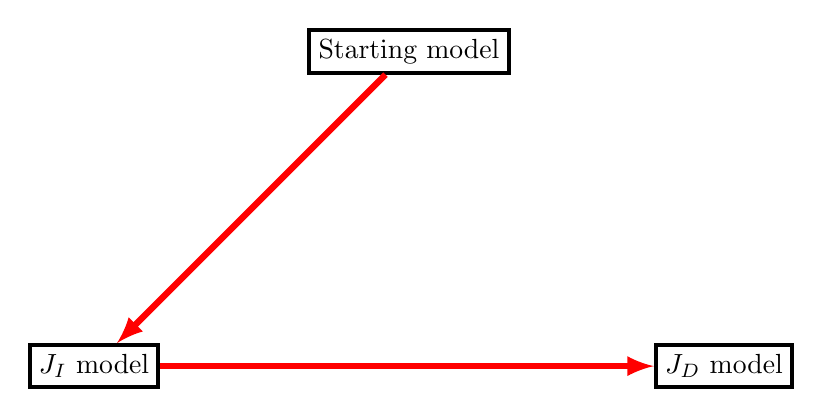
\begin{tikzpicture}
        \path (0,0)  node[RectObject] (x) {Starting model}; 
        \path (4,-4) node[RectObject] (y) {$J_D$ model};
        \path (-4,-4)  node[RectObject] (z) {$J_I$ model};
        \draw[rarrow] (x) -> (z);
        \draw[rarrow] (z) -> (y);
      \end{tikzpicture}
    \end{center}
\end{frame} 

\inputdir{workshop}


\begin{frame}
  \vspace{.63cm}
    \begin{flushleft}
      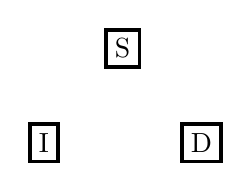
\begin{tikzpicture}
        \path (0,0)  node[RectObject] (x) {{\red S}}; 
        \path (1.,-1.2) node[RectObject] (y) {D};
        \path (-1,-1.2)  node[RectObject] (z) {I};
      \end{tikzpicture}
    \end{flushleft}
  \vspace{-1cm}
 \plot{image-wtomo-cip}{width=\textwidth}{}
\end{frame}




\begin{frame}
  \vspace{.63cm}
    \begin{flushleft}
      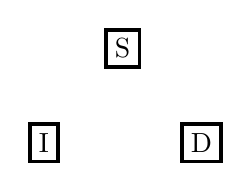
\begin{tikzpicture}
        \path (0,0)  node[RectObject] (x) {{\red S}}; 
        \path (1.,-1.2) node[RectObject] (y) {D};
        \path (-1,-1.2)  node[RectObject] (z) {I};
      \end{tikzpicture}
    \end{flushleft}
  \vspace{-1cm}
 \plot{image-winit}{width=\textwidth}{}
\end{frame}


\begin{frame}
  \vspace{.63cm}
    \begin{flushleft}
      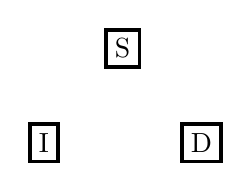
\begin{tikzpicture}
        \path (0,0)  node[RectObject] (x) {S}; 
        \path (1.,-1.2) node[RectObject] (y) {D};
        \path (-1,-1.2)  node[RectObject] (z) {{\red I}};
      \end{tikzpicture}
    \end{flushleft}
  \vspace{-1cm}
 \plot{image-wtomo}{width=\textwidth}{}
\end{frame}

\begin{frame}
  \vspace{.63cm}
    \begin{flushleft}
      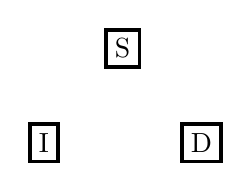
\begin{tikzpicture}
        \path (0,0)  node[RectObject] (x) {S}; 
        \path (1.,-1.2) node[RectObject] (y) {{\red D}};
        \path (-1,-1.2)  node[RectObject] (z) {I};
      \end{tikzpicture}
    \end{flushleft}
  \vspace{-1cm}
 \plot{image-wfwi}{width=\textwidth}{}
\end{frame}





\begin{frame}
  \vspace{.63cm}
    \begin{flushleft}
      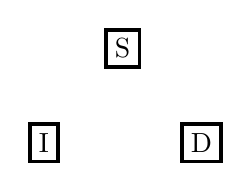
\begin{tikzpicture}
        \path (0,0)  node[RectObject] (x) {\red{S}}; 
        \path (1.,-1.2) node[RectObject] (y) {D};
        \path (-1,-1.2)  node[RectObject] (z) {I};
      \end{tikzpicture}
    \end{flushleft}
  \vspace{-1cm}
 \plot{anglex-image-winit}{width=\textwidth}{}
\end{frame}


\begin{frame}
  \vspace{.63cm}
    \begin{flushleft}
      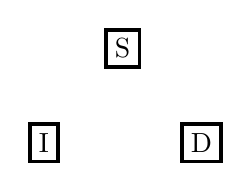
\begin{tikzpicture}
        \path (0,0)  node[RectObject] (x) {S}; 
        \path (1.,-1.2) node[RectObject] (y) {D};
        \path (-1,-1.2)  node[RectObject] (z) {\red{I}};
      \end{tikzpicture}
    \end{flushleft}
  \vspace{-1cm}
 \plot{anglex-image-wtomo}{width=\textwidth}{}
\end{frame}

\begin{frame}
  \vspace{.63cm}
    \begin{flushleft}
      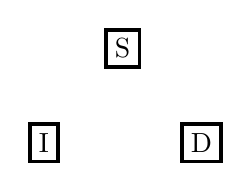
\begin{tikzpicture}
        \path (0,0)  node[RectObject] (x) {S}; 
        \path (1.,-1.2) node[RectObject] (y) {\red{D}};
        \path (-1,-1.2)  node[RectObject] (z) {I};
      \end{tikzpicture}
    \end{flushleft}
  \vspace{-1cm}
 \plot{anglex-image-wfwi}{width=\textwidth}{}
\end{frame}









\begin{frame}
  \vspace{.63cm}
    \begin{flushleft}
      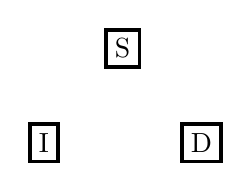
\begin{tikzpicture}
        \path (0,0)  node[RectObject] (x) {\red{S}}; 
        \path (1.,-1.2) node[RectObject] (y) {D};
        \path (-1,-1.2)  node[RectObject] (z) {I};
      \end{tikzpicture}
    \end{flushleft}
  \vspace{-1cm}
 \plot{vel-winit}{width=\textwidth}{}
\end{frame}


\begin{frame}
  \vspace{.63cm}
    \begin{flushleft}
      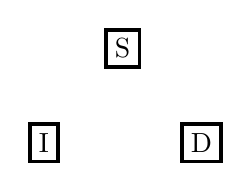
\begin{tikzpicture}
        \path (0,0)  node[RectObject] (x) {S}; 
        \path (1.,-1.2) node[RectObject] (y) {D};
        \path (-1,-1.2)  node[RectObject] (z) {\red{I}};
      \end{tikzpicture}
    \end{flushleft}
  \vspace{-1cm}
 \plot{vel-wtomo}{width=\textwidth}{}
\end{frame}

\begin{frame}
  \vspace{.63cm}
    \begin{flushleft}
      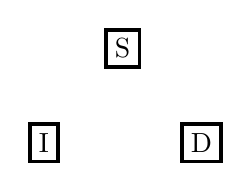
\begin{tikzpicture}
        \path (0,0)  node[RectObject] (x) {S}; 
        \path (1.,-1.2) node[RectObject] (y) {\red{D}};
        \path (-1,-1.2)  node[RectObject] (z) {I};
      \end{tikzpicture}
    \end{flushleft}
  \vspace{-1cm}
 \plot{vel-wfwi}{width=\textwidth}{}
\end{frame}

\begin{frame}
\end{frame}



\begin{frame}\frametitle{conclusions}
  \begin{columns}
    \column{0.5\textwidth}
      \itab{cost}
    \column{0.5\textwidth}
      \itab{CIP}
  \end{columns}
  \vfill
  \pause
  \begin{columns}
    \column{0.5\textwidth}
      \itab{illumination}
    \column{0.5\textwidth}
      \itab{PSF penalty}
  \end{columns}
  \vfill
  \pause
  \begin{columns}
    \column{0.5\textwidth}
      \itab{resolution}
    \column{0.5\textwidth}
      \itab{data-domain WT}
  \end{columns}
  \vfill
\end{frame}


\begin{frame}\frametitle{acknowledgments}
\cen{Bruce VerWest, Gerhard Pratt, Yuting Duan, Tariq Alkhalifah, and Zedong Wu.}
\end{frame}

\begin{frame}\frametitle{acknowledgments}
\begin{figure}[p]
    \includegraphics[width=0.3\textwidth]{cgg}
\end{figure}
\end{frame}

\inputdir{.}
\begin{frame}\frametitle{acknowledgments}
  \plot{thank2}{height=.9\textheight}{}
\end{frame}


\begin{frame}
\end{frame}

